\documentclass[12pt]{article}
%\usepackage[cp1251]{inputenc}
\usepackage[utf8]{inputenc}
\usepackage[bulgarian]{babel}
\usepackage{amssymb,amsmath,amsfonts,amstext,amscd,latexsym}
\usepackage{graphicx}
\usepackage{upgreek}
\usepackage{amsmath}
\usepackage[colorinlistoftodos]{todonotes}
\usepackage{systeme}
\usepackage[geometry]{ifsym}
\usepackage{listings}
\usepackage{float}
\usepackage{color}

\begin{document}
	\begin{titlepage}	
		\newcommand{\HRule}{\rule{\linewidth}{0.5mm}} % Defines a new command for the horizontal lines, change thickness here
		\begin{center}
		\textsc{\LARGE Софийски университет }\\[0.3cm]
		\textsc{\LARGE "Св. Климент Охридски" }\\[0.3cm]
		\textsc{\Large Факултет по математика и информатика }\\[0.2cm]
		%\fontsize{size}{baselineskip}
		
		{\fontsize{12}{18}\selectfont \bf МАШИННО САМООБУЧЕНИЕ}\vspace{15pt}\newline спец. Изкуствен интелект, I курс, зимен семестър \newline учебна година 2024/2025
		\vspace{30pt}
		
		
		
		
		
		\begin{minipage}{0.4\textwidth}
			\begin{flushleft}\large
				\emph{Изготвил:} \\
				Кристиян Симов \\ 
				фак. номер 4MI3400288
			\end{flushleft}
		\end{minipage}
		~
		%\begin{flushleft}
		\begin{minipage}{0.4\textwidth}
			\begin{flushright}
				\large
				\emph{Дата:}\\
				18. 11. 2024 г. % Попълнете датата на предаване
				\\София 
			\end{flushright}
		\end{minipage}\\[1cm]
		%\end{flushleft}
		\bigskip
		{\large \textbf{Домашна работа \textnumero 3}}\\[1cm] % Date, change the \today to a set date if you want to be precise
		%\includegraphics{rsz_sofia_university_logo.png}\\[1cm] 
		
\includegraphics{logo_su_no_text.png}\\[1cm]
		\vfill % Fill the rest of the page with whitespace
		\end{center}
	\end{titlepage}
	
	
	
	\tableofcontents
	
	
	
	\newpage
	
	\section{Решение на задача \textnumero 1}
	
	Единствената нужна промяна на алгоритъм \textbf{НАУЧИ-ЕДНО-ПРАВИЛО} от Лекция 5 Табл.5-2, която ще позволи той да работи коректно ако някой от атрибутите с непрекъснати стойности, е да прибавим генериране (вътре в цикъла "за всяка хипотеза $h$ от \textit{Кандидат-хипотези}" от първа точка) на ограничения $c$ от вида $A_{i} > v_{i,j}$ и $A_{i} <= v_{i,j}$, $j \in \{1, n'\}$ за всеки непрекъснат атрибут $A_{i}$, където $v_{i,1},...,v_{i,n'}$ са намерените възможни гранични стойности за атрибута $A_i$, чрез сортиране на всички $n'$ на брой примери, които се покриват от текущата хипотеза $h$ в цикъла (в началото това коректно са всички примери, тъй като h e най-общата хипотеза, покриваща всичките $n$ примера, т.е $n' = n$) и намирането на средно аритметичното на всеки две съседни стойности по $A_{i}$ в сортираната последователност $a_{i1},..,a_{in'}$. 
	\newline\newline Така получаваме $v_{i,1} = \frac{a_{i1}+a_{i2}}{2},...,v_{i,n'} = \frac{a_{i(n'-1)}+a_{in'}}{2}$ и след това допълнителните възможни ограничения $(A_{i} > v_{i,j})$ и $(A_{i} <= v_{i,j})$, $j \in \{1, n'\}$, които искахме да генерираме, тъй като сред тях е възможно да изберем (ако някое от тях има най-добра евристика) новата конюнкция към правилото което строим.
	Това правим за всеки непрекъснат атрибут $A_{i}$. Тоест вече избираме $c$ от обединението на множеството \textit{Всички-ограничения} (предварително генерираните ограничения за дискретните атрибути) и всички така генерирани допълнителни правила за непрекъснатите атрибути.  Това правим за всяка хипотеза от цикъла, защото ако тя покрива различни примери, това променя вида на сортираната последователност и съответно изчисленията при средните стойности. Всяка спецификация чрез кое да е ограничение би могла потенциално да промени множеството от покриваните примери.
	

	\newpage
	
	\section{Решение на задача \textnumero 2}
	
	Нека има два персептрона ($A$ и $B$), чиято повърхност на решение се
	определя с формулата:
	\subparagraph{}
	$w_{0} + w_{1}x_{1} + w_{2}x_{2} > 0$
	\newline\newline\newline
	Нека персептрон $A$ има следните стойности на теглата:
	\subparagraph{}
	$w_{0} = 1, w_{1} = 2, w_{2} = 1$
	\newline\newline
	Нека персептрон $B$ има следните стойности на теглата:
	\subparagraph{}
	$w_{0} = 0, w_{1} = 2, w_{2} = 1$
	\newline\newline\newline
	В случая имаме $x_{1}$ и $x_{2}$ (два входа). Следователно за персептрони $A$ и $B$ n-мерните хиперплоскости, които отделят n-мерното пространство на примерите, представляват прави в двумерно пространство:\newpage
	\begin{figure}[H]
		\centering
		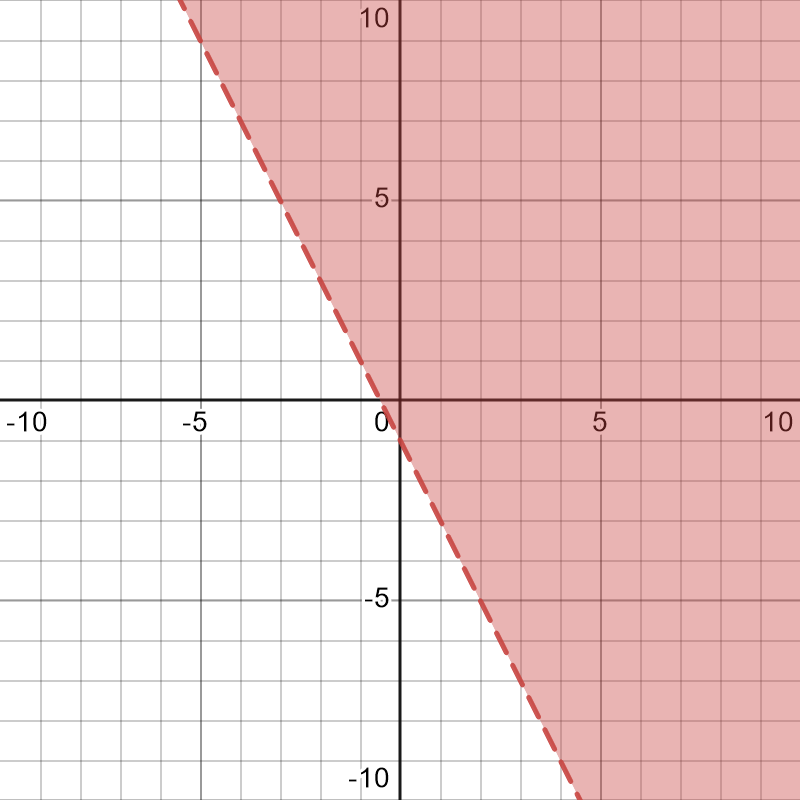
\includegraphics[width=140mm]{desmos-graph.png} 
		\caption{Персептрон $A$. В червен пунктир виждаме графиката на правата $1 + 2x_{1} + x_{2} = 0$, която отделя пространството, а със светло червено е запълнено множеството от стойности които са решение на неравенството $1 + 2x_{1} + x_{2} > 0$}
	\end{figure}
	\newpage
	\begin{figure}[H]
		\centering
		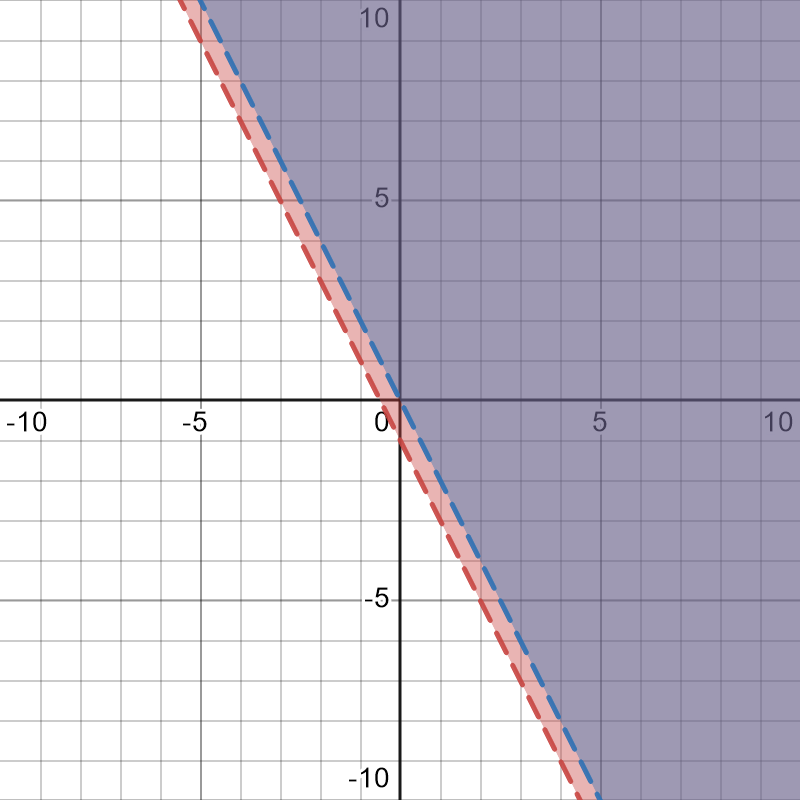
\includegraphics[width=140mm]{desmos-graph(1).png} 
		\caption{Персептрони $A$ и $B$. Върху предходната Фигура 1 е нанесена със син пунктир графиката на правата $2x_{1} + x_{2} = 0$, която отделя пространството, а със светло син е запълнено множеството от стойности които са решение на неравенството $2x_{1} + x_{2} > 0$. Виждаме, че то е подмножество на множеството от решения на оцветената в светло червено област от решения на неравенството $1 + 2x_{1} + x_{2} > 0$. Това означава, че всяка точка от синята област е решение за червената, но обратното не е в сила. Следователно $A >_{g}$ B. $\square$}
	\end{figure}

		
	\newpage
	
	\section{Решение на задача \textnumero 3}
	
	\begin{figure}[H]
		\centering
		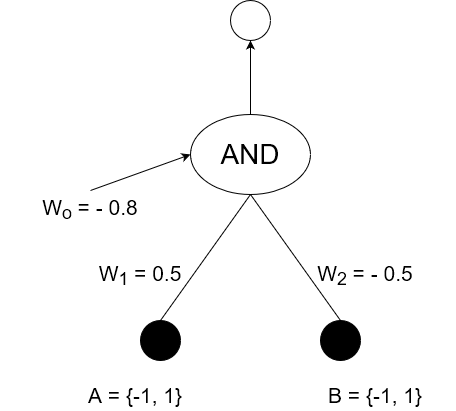
\includegraphics[width=150mm]{Untitled1.png} 
		\caption{a) $A \land \lnot B$}
	\end{figure}
	
	\begin{figure}[H]
		\centering
		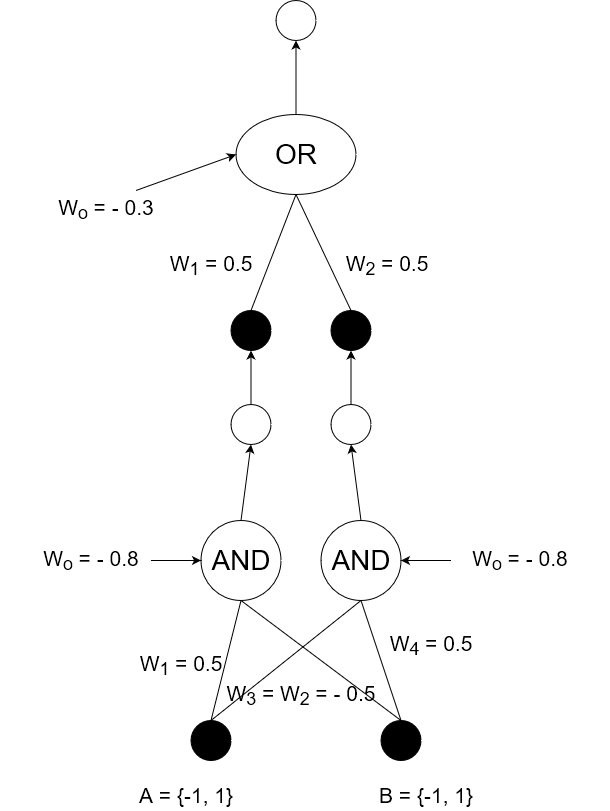
\includegraphics[width=140mm]{Untitled2.png} 
		\caption{b) $(A \land \lnot B) \lor (\lnot A \land B)$}
	\end{figure}
	
	
		
	\newpage
	
	\section{Решение на задача \textnumero 4}
	
	Ще изведем правилото за обучение чрез градиентното спускане на един линеен възел, чийто изход $o$ се задава от формулата:
	\subparagraph{}
	$o = w_{0} + w_{1}x_{1} + w_{1}x_{1}^2 + ... + w_{n}x_{n} + w_{n}x_{n}^2 $
	\newline\newline\newline
	Правилото за обучение чрез градиентното спускане в покомпонентен вид е следното:
	\subparagraph{}
	$w_{i} \leftarrow w_{i} + \Updelta w_{i} \text{, където } \Updelta w_{i} = - \eta \frac{\delta E}{\delta w_{i}}$
	\newline\newline\newline
	Пресмятаме частната производна $\frac{\delta E}{\delta w_{i}}$, компонент на вектора от производни (градиента), указващ посоката на най-бързо изкачване:
	\subparagraph{}
	$\displaystyle\frac{\delta E}{\delta w_{i}} = \frac{\delta}{\delta w_{i}}\frac{1}{2}\sum_{d \in D}(t_{d} - o_{d})^2 = \frac{1}{2} \sum_{d \in D}2(t_{d} - o_{d})\frac{\delta}{\delta w_{i}}(t_{d} - o_{d}) =$  \newline \subparagraph{}$ = \displaystyle \sum_{d \in D}(t_{d} - o_{d})\frac{\delta}{\delta w_{i}}(t_{d} - \vec{w}  \vec{x_{d}}) = \sum_{d \in D}(t_{d} - o_{d})(-x_{id} - x_{id}^2)$
	\newline\newline
	Пресмятаме правилото за обновяване на тегла $\Updelta w_{i}$, замествайки с $\frac{\delta E}{\delta w_{i}}$:
	\subparagraph{}
	$\Updelta w_{i} = - \eta \frac{\delta E}{\delta w_{i}} = - \eta \displaystyle\sum_{d \in D}(t_{d} - o_{d})(-x_{id} - x_{id}^2) = \eta \displaystyle\sum_{d \in D}(t_{d} - o_{d})(x_{id} + x_{id}^2) $
	\newline\newline\newline
	Така в крайна сметка, замествайки последното правило в предпоследното покомпонентно правило, получаваме правилото:
	\subparagraph{}
	$w_{i} \leftarrow w_{i} + \Updelta w_{i} \text{, където } \Updelta w_{i} = \eta \displaystyle\sum_{d \in D}(t_{d} - o_{d})(x_{id} + x_{id}^2),$
	\newline\newline\newline в което $x_{id}$ означава входния компонент $x_{i}$ на обучаващия пример $d$. $\square$
	


	
\end{document}